\chapter{Related work}
\label{chap:rel_work}
%TODO When done, fix this
This chapter discusses the relevant literature and state of the art for this thesis; the literature is grouped into \FetchStoredCounterValue{section} sections. In \autoref{section:routing_rel_work}, the routing algorithms for transport are discussed. Next, we examine the data models used in public transport (\autoref{section:data_model_rel_work}). Further, we look at existing ontologies for transportation in \autoref{section:ontologies_rel_work}.

\section{Transport Routing Algorithms }\label{section:routing_rel_work}

\subsection{Type of Queries}
In \glsfmtshort{pt}, different sorts of Queries are possible. Whereas in road networks, we are only interested in the shortest path, we are generally more interested in supporting multiple criteria. 
\begin{itemize}
    \item \glsxtrfull{eat} query is the simplest, which takes a departure time as an additional input and returns a journey that arrives as early as possible.
    \item \glsxtrfull{mc} is an extension. It takes the number of transfers into account. This query results in a set of journeys.
    \item Profile query determines all optimal journeys departing during a given period.
\end{itemize}

We are most interested in Earliest arrival queries.
% include timeline image
\subsection{History of routing algoritms}
\begin{figure}[H]
\resizebox{\textwidth}{!}{%
    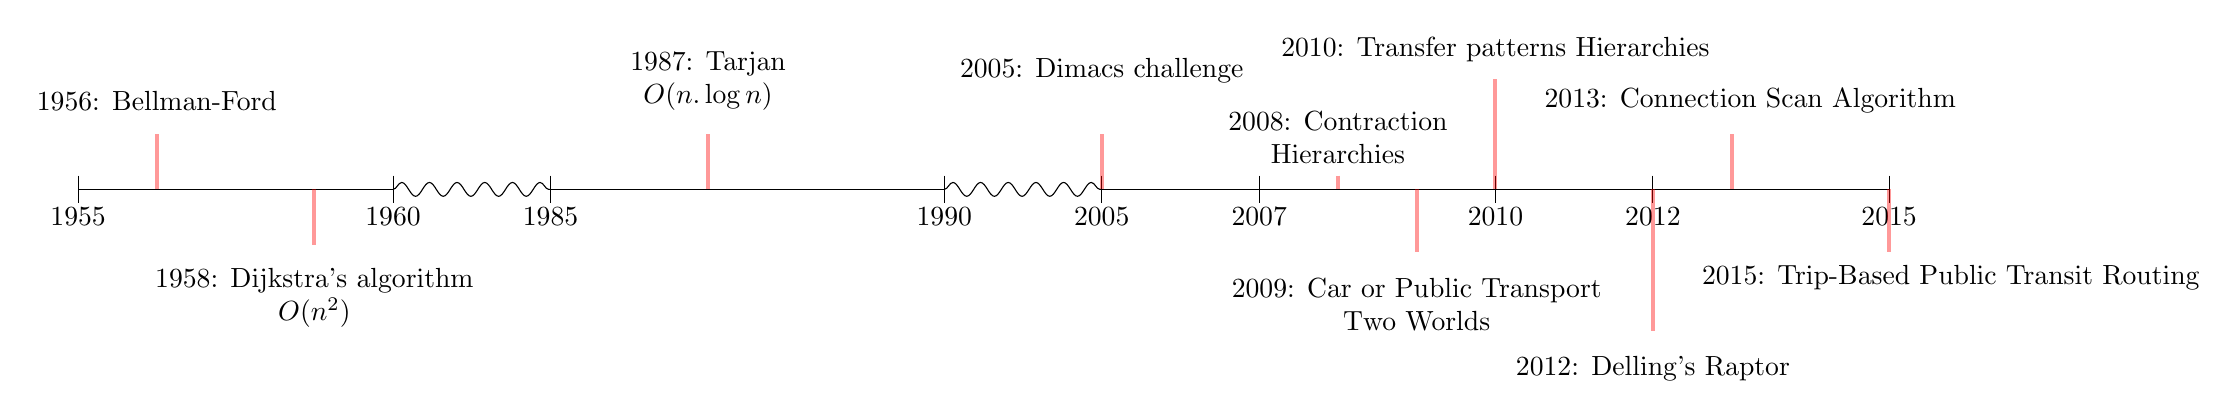
\begin{tikzpicture}
    % Draw a horizontal line
    \draw (0,0) -- (4,0);
    \draw (6,0) -- (11,0);
    \draw (13,0) -- (23,0);
    
    % draw vertical lines
    \foreach \x in {0,4,6,11,13,18,23,15,20}
    \draw (\x cm,5pt) -- (\x cm,-5pt);
    
    \foreach \x in {1,8,13,21}
    \draw[line width=0.5mm, red, opacity=0.4 ] (\x cm,20pt) -- (\x cm,0);
    
    \foreach \x in {3}
    \draw[line width=0.5mm, red, opacity=0.4 ] (\x cm,0) -- (\x cm,-20pt);
    
    % draw nodes to add events
    \draw (0,0) node[below=3pt] {1955};
    \draw (4,0) node[below=3pt] {1960};
    \draw (6,0) node[below=3pt] {1985};
    \draw (11,0) node[below=3pt] {1990};
    \draw (13,0) node[below=3pt] {2005};
    \draw (15,0) node[below=3pt] {2007};
    \draw (18,0) node[below=3pt] {2010};
    \draw (20,0) node[below=3pt] {2012};
    \draw (23,0) node[below=3pt] {2015};
    
    \draw (1,0) node[above=25pt] {1956: Bellman-Ford};
    
    \draw (3,0) node[below=25pt, align=center] {1958: Dijkstra’s algorithm\\ $O(n^2)$};
    
    \draw (8,0) node[above=25pt, align=center] {1987: Tarjan\\ $O(n.\log{n})$};
    
    \draw (13,0) node[above=35pt] {2005: Dimacs challenge};
    
    \draw (16,0) node[above=0.2cm, align=center] {2008: Contraction \\Hierarchies};
    \draw[line width=0.5mm, red, opacity=0.4 ] (16 cm,5pt) -- (16 cm,0);
    
    \draw (17,0) node[below=1cm, align=center] {2009: Car or Public Transport\\ Two Worlds};
    \draw[line width=0.5mm, red , opacity=0.4] (17 cm,0) -- (17 cm,-0.8cm);
    
    
    \draw (18,0) node[above=1.5cm] {2010: Transfer patterns Hierarchies};
    \draw[line width=0.5mm, red , opacity=0.4] (18 cm,1.4cm) -- (18 cm,0);
    
    \draw (20,0) node[below=2cm] {2012: Delling’s Raptor};
    \draw[line width=0.5mm, red, opacity=0.4] (20 cm,0) -- (20 cm,-1.8cm);
    
    \draw (21,0) node[above=32pt,right=-2.5 cm] {2013: Connection Scan Algorithm};

    \draw (23,0) node[below=32pt,right=-2.5 cm] {2015: Trip-Based Public Transit Routing};
    \draw[line width=0.5mm, red, opacity=0.4] (23 cm,0) -- (23 cm,-0.8cm);
    
    
    \draw[decoration={snake},decorate] (4,0) -- (6,0);
    \draw[decoration={snake},decorate] (11,0) -- (13,0);
    \end{tikzpicture}
    }
    \caption{Timeline describing the developments in route planning. The crossed parts represent}
    \label{fig:timeline}
\end{figure}

This section discusses the state of the art and history of public transport planning. Therefore, a tiny timeline (\autoref{fig:timeline}) was constructed to visualize some important milestones explained below. As seen in the timeline, most advances were made after 2009.

\subsection{Dijkstra}
% add some dijkstra algo workings, easy
The milestones between 1956 and 2008 did not apply to PT routing but focused on normal road networks. Among these milestones was the Dijkstra algorithm, published in 1958. This was the first big improvement but had a time complexity of $O(n^2)$. An improved version was proposed almost 30 years later, in 1987. It has a complexity of $O(n*\log(n))$ and is the version of the Dijkstra algorithm learnt at schools.% It works by initializing every node to $\infty$ except the source node, which is initialized to $0$. Then, every edge of the source node is visited. 
\subsection{Dimacs challenge}
No significant improvements for route planners were made until 2005. The road network of the US was published as part of the 9th Dimacs challenge \cite{noauthor_9th_2017}. A big deal for researchers, now they had an extensive dataset to test on. Many speedup techniques, mainly pruning techniques, were devised for the Dijkstra algorithms. But this was still inapplicable to \glsxtrshort{pt}.

\subsection{Car or Public Transport: Two Worlds}
In 2009, a paper, Car or Public Transport: Two Worlds \cite{bast_car_2009}, stated, “There are two kinds of people: those who travel by car, and those who use public transport.”. They argued that the worlds differed, although both problems could be represented as a directed graph. For PT, we must deal with timetable schedules in addition to this spatial information.

The article covers five big “tricks of the trade” for fast routing on transportation: Bidirectional search, exploiting hierarchy, graph contraction, goal direction and distance tables. It explains why the trick works on road networks but falls short on \glsxtrshort{pt}.

\subsubsection{Bidirectional search}
A simple approach to improve Dijkstra is to search from the source node but simultaneously do a backward search from the target node. This reduces the search space by half and can be quickly done for road networks since both nodes associated with the station are known. The idea is not very practical but is critical to implementing other speedup techniques.

For \glsxtrshort{pt}, this idea adds a lot of complexity since, in a time-expanded graph, we know the target station but not the target node. A solution is to do a backward set of all nodes associated with the end station.
\subsubsection{Exploiting hierarchy}
Roads have different levels of importance: think of motorways, national highways, and minor roads. The simple routing heuristic exploits this hierarchy. When we are within a certain distance of the target and source node, we take all streets into account. In the other case, we use only high-level roads, reducing the total number of explored nodes. This comes with some loss of exactness.

However, this technique can be even slower in large municipal areas because the hierarchy is absent. The tram, metro and bus are equally important. A hierarchy begins to appear only when travelling long distances between cities. 
\subsubsection{Graph contraction}
For aesthetics, curved reads were replaced by multiple straight lines. This resulted in more edges and nodes, so researchers quickly reverted this. This is a contraction, and the resulting edge is called a shortcut. This even works in hierarchies because higher levels have junctions that would lead to lower levels. So, these junctions could be neglected and replaced by a shortcut. 

Similar to the previous problem, the hierarchy is absent. This technique does not work for \glsfmtshort{pt} in a large municipal area.
\subsubsection{Goal direction}
The Dijkstra algorithm is augmented with a heuristic, which leads to an algorithm like $ A*$. The chosen heuristic dramatically influences the performance.

The problem is the lack of algorithms for local searches on \glsfmtshort{pt} networks, and this causes quadratic precomputations.
\subsubsection{Distance tables}
As the name suggests, this table contains the calculated distances between all pairs of nodes in the graph. It’s an extreme precomputation, but query times will be nearly instantaneous. 

In \glsxtrshort{pt}, we do not have efficient algorithms for local searches.
\subsubsection{Conclusion}
The paper identifies two big problems\footnote{These were problems at the time, and solutions have been proposed since then.}. 
\begin{enumerate}
    \item How to achieve speed-ups despite lack of hierarchy
    \item How to compute shortest paths to all nodes in a local neighbourhood efficiently.
\end{enumerate}
\subsection{Transfer patterns}
Transfer patterns are considered the first algorithm for PT that solves queries in an order of a few milliseconds and on a transport network with a poor structure. 

Transfer patterns describe a method using a journey planning algorithm to pre-calculate all the unique journeys for the entire graph \cite{bast_fast_2010}. This means we can look up the schedule matching that journey when a real-time query comes in. In this case, the server can give fast query responses, but the pre-calculations can cause a computational burden. For example, the authors used a cluster of Opteron and Xeon-based 64-bit servers for their CPP implementation. Although the exact number of compute nodes is not mentioned in the paper \cite{bast_fast_2010}. They say the needed core hours are around 3000, so running on a single core would take about four months to finish.

For the most simplistic description, we need to return to the scenario described in the introduction: assume you’re in your first year and want to go to the city centre. You do not have a smartphone or internet, only a printed schedule book. A local points out that there are only two reasonable options \begin{enumerate}
    \item Take a tram from A to C, then transfer at C to a bus to B.
    \item Take an infrequently run, direct bus from A to B.
\end{enumerate} 
Note that this is compact information, but it makes searching in the printed schedule much faster since any other trip will not be faster, so it can safely be discarded. \cite{noauthor_update_nodate}


Key ideas:
\begin{itemize}
    \item Of the shortest paths, many share the same transfer pattern.
    \item Direct connections that do not require a change of vehicle can be looked up rather quickly. 
\end{itemize}
A simple algorithm for transfer patterns illustrates the key ideas and consists of 3 parts but has quadratic precomputation complexity. A more optimized algorithm is described in the paper \cite{bast_fast_2010}.
\subsubsection{Graph}
The algorithm works on a time-expanded graph with three kinds of nodes: a departure node, an arrival node and a transfer node. Each node carries the time and the station to which it belongs. Like in \autoref{fig:transferel}.
\begin{figure}[H]
\begin{minipage}{.45\textwidth}

\centering
\resizebox{0.5\linewidth}{!}{%
    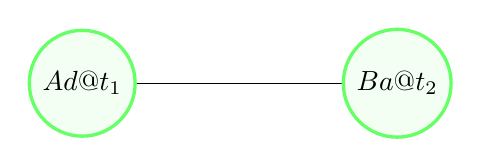
\begin{tikzpicture}[
roundnode/.style={circle, draw=green!60, fill=green!5, very thick, minimum size=8mm},
]
    
    \draw (0,0) -- (4,0);
    
    \draw (4,0) node[align=center,roundnode] {$Ba@t_2$};

    \draw (0,0) node[align=center,roundnode] {$Ad@t_1$};
    
    \end{tikzpicture}
%
}%
    \caption{An elementary connection betweens stations A and B, d stands for departure and a for arrival, $@t_i$ denotes the time the vehicle departs, arrives are waits (transfer)}
    \label{fig:transferel}

\end{minipage}\hspace{.1\textwidth}
\begin{minipage}{.45\textwidth}
\centering
\resizebox{0.5\linewidth}{!}{%
    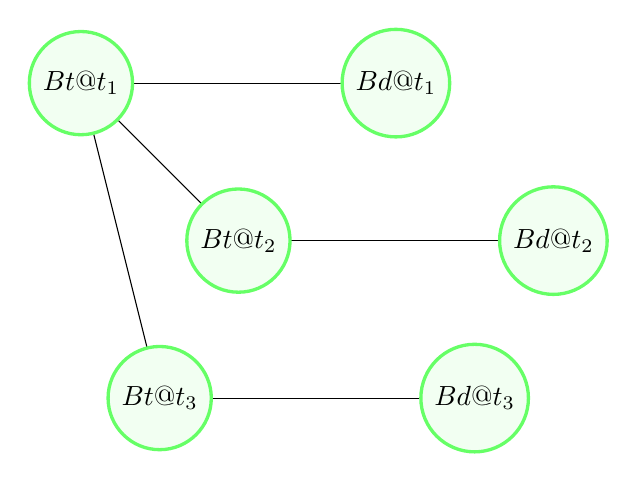
\begin{tikzpicture}[
roundnode/.style={circle, draw=green!60, fill=green!5, very thick, minimum size=8mm},
]
    
    \draw (0,0) -- (4,0);
    \draw (0,0) -- (2,-2);
    \draw (0,0) -- (1,-4);
    \draw (1,-4) -- (5,-4);
    \draw (2,-2) -- (6,-2);
    
    \draw (0,0) node[align=center,roundnode] {$Bt@t_1$};

    \draw (4,0) node[align=center,roundnode] {$Bd@t_1$};


    
    \draw (2,-2) node[align=center,roundnode] {$Bt@t_2$};

    \draw (6,-2) node[align=center,roundnode] {$Bd@t_2$};

    \draw (1,-4) node[align=center,roundnode] {$Bt@t_3$};

    \draw (5,-4) node[align=center,roundnode] {$Bd@t_3$};
    \end{tikzpicture}
%
}%
    \caption{An transfer, with an waiting chain}
    \label{fig:transferpatterntransfer}

\end{minipage}
\end{figure}
\subsubsection{Fast direct-connections queries}
This part is only for direct connections, meaning a maximal path in the graph without transfer nodes.

\begin{enumerate}
    \item Precompute all maximal paths in the graph without transfer nodes. Group them in lines that share the same sequence of stations. This creates an ordered timetable for a particular line.
    \item Precompute for each station the sorted list of lines in which the station occurs and its position(s) on the line. This creates a lookup table, which can be used to find timetables of lines stations share.
    \item To answer a direct connection query, use the precomputed sorted list of the departure and arrival stations. See if they share a line with the departure station, which has a lower position than the arrival station. Using the timetables of the found lines, determine the earliest arrival time.
\end{enumerate}
\subsubsection{Transfer patterns precomputation}
This step is crucial to speed up the search process during actual queries. 

 Starting with the following definition\cite{bast_fast_2010} of a transfer pattern, which is also visualized by \autoref{fig:transferpatternexampletransferpattern}
\begin{quote}
    For any path, consider the subsequence of nodes formed by the first node, each arrival node whose successor is a transfer node, and the last node. The sequence of stations of these nodes is the transfer pattern of the path.
\end{quote}
\begin{figure}[H]

\centering
\resizebox{0.6\linewidth}{!}{%
    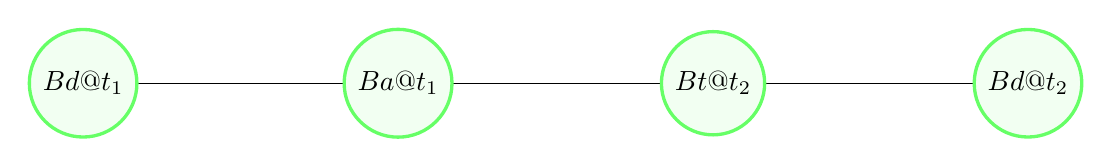
\begin{tikzpicture}[
roundnode/.style={circle, draw=green!60, fill=green!5, very thick, minimum size=7mm},
]

    \draw (0,0) node[align=center,roundnode] {$Bd@t_1$} -- (4,0) node[align=center,roundnode] {$Ba@t_1$} -- (8,0) node[align=center,roundnode] {$Bt@t_2$} -- (12,0) node[align=center,roundnode] {$Bd@t_2$};
    \end{tikzpicture}
%
}%
    \caption{A transfer pattern}
    \label{fig:transferpatternexampletransferpattern}

\end{figure}
More simply put, a transfer pattern is where a change of vehicle or transfer occurs. 

Now that we know what a transfer pattern is, we can define an optimal set of transfer patterns for a pair of stations (a,b). It is a set of transfer patterns with an optimal set of connections for all queries whose transfer patterns are contained in S. In turn, each element of the set is the transfer pattern of an optimal connection for a query at some time. 

From a given source station A, compute optimal sets of transfer patterns to all station B that are reachable. 
\begin{enumerate}
    \item We start labels with zero cost at all transfer nodes at source node/station A and run a multi-criteria variant of Dijkstra on them.
    \item For every station B, choose optimal connections with the arrival chain algorithm.
    \begin{enumerate}
        \item Select a dominant subset in the set of labels
    \end{enumerate}
    \item Trace back the paths of all labels selected in Step 2. Create the DAG of transfer patterns of these paths by traversing them from source A.r
\end{enumerate}
\subsubsection{Query graph construction and evaluation}
We start from the precomputed transfer pattern DAG generated in the previous step.

Assume we have a query from station A to station B.
\begin{enumerate}
    \item Fetch the DAG of station A.
    \item Search for the target station B. Add at each each successor node to the graph.
    \item Recursively repeat the previous step for each successor station that is not A.
\end{enumerate}
Then, run Dijkstra on search on the query graph.

\subsubsection{Frequency-Based Search for Public Transit}
An improvement in transfer patterns preprocessing by a factor of 60. This paper\cite{bast_frequency-based_2014} assumes that most connections in public transport networks are run periodically (e.g. a tram every 10 mins). So, it is more efficient to store the frequency and time range. They propose a compression scheme for timetable data of public transportation networks where synchronized departures are joined into single frequency-based labels.
\subsubsection{Scalable transfer patterns}
The paper on Scalable transfer patterns \cite{bast_scalable_2015} identifies two criteria (the space consumption of the precomputed auxiliary data is large, and the preprocessing time is enormous) in which transfer patterns are lacking. Furthermore, the scalability of transfer patterns is addressed by introducing a new scheme based on clustering the network for Transfer Patterns precomputation and query graph construction that allows interactive query times for massive transit networks with manageable preprocessing times and space consumption. 
\subsection{\glsfmtfull{csa}}
\glsxtrfull{csa} \cite{dibbelt_intriguingly_2013} organizes its data as a single array of connections, scanned only once per query. It supports the earliest arrival and multiple criteria. Another characteristic is that it is not graph-based, like \glsxtrshort{raptor}. But unlike \glsfmtshort{raptor}, it is centred around elementary connections.

The algorithm builds on the following property that a connection is readable if \begin{enumerate}
    \item You are travelling on a preceding connection of the same trip. 
    \item You are at the departing stop of the connection.
\end{enumerate}
This property is also encoded into the time-dependent models\cite{pyrga_efficient_2008}, but Dijkstra is inefficient on these graphs due to priority queues and suboptimal memory accesses. 
\subsubsection{Algorithm}
The \glsxtrshort{csa} algorithm is straightforward. 

The timetable connections are assembled into an array and sorted by departure time. Each stop is given a label representing its earliest arrival time. Initially, they are set to infinity, except for the source stop, which is set to our desired departure time. Then, all connections in the array are scanned. If a connection can be reached and the arrival time (the connection’s label) can be improved, we relax the connection by updating its label. 

\subsubsection{Binary search}
Scanning the entire array is wasteful. All connections departing before our departure time are unnecessary to scan since they can never be reached. To find the relevant connection, we perform a binary search. 
\subsection{Trip-based public transit routing}
Trip-based public transit routing uses trips and the transfers between them as its fundamental building blocks. 

A basic overview of the algorithm is as follows:
\begin{enumerate}
    \item Label trips with the stops at which they are boarded.
    \item Scan a precomputed list of transfers; new trips that can be reached are again labelled with stops.
    \item If a trip reaches the destination, we add the journey to the result set.
    \item algorithm terminates when all optimal journeys are found.
\end{enumerate}
\subsubsection{Preprocessing}
We precompute the possible transfers to speed up queries. It consists of two steps:
\begin{enumerate}
    \item initial computation: \begin{enumerate}
        \item For each stop of all trips, find all lines passing through the stop, and all stops reachable by a direct footpath.
        \item Iterate over all lines and search the first trip such that arrival time + time to footpath is smaller than the departure time.
    \end{enumerate}
    \item Reduction. We discard transfers that aren’t useful \begin{enumerate}
        \item Remove U-turn transfers. These transfers to a trip X that, in turn, passed through a stop in the original trip.
        \item Reduce the number of transfers by analyzing which transfers lead to improved arrival times.
    \end{enumerate}
    
\end{enumerate}
\subsubsection{Earliest arrival time query}

\subsection{\glsfmtfull{raptor}}
\glsxtrfull{raptor} is a graph-based algorithm that solves queries in rounds. Round K computes the fastest way of getting to every stop with at most k - 1 transfers or k trips.

\begin{enumerate}
    \item Each node gets a multilabel. $(\tau_0,...,\tau_k)$ with $\tau_i$ representing the earliest arrival time in $i$ trips. We init all arrival times in each label with $\infty$. Except for the departing node, where $\tau_0$ is set to the depart time of our search criteria.
    \item For each round $k$ our goal is to compute $\tau_k$. This happens in three stages:\begin{enumerate}
        \item Set the earliest arrival time k ($\tau_k$) to that of iets predescor ($\tau_{k-1}$). This is an upper bound since we are not interested in slower stop times than the previous round.
        \item We iterate over the routes. We calculate the earliest trip we can take for each stop $p$ on the route $r$. This does not always exist. We search stops along the route $r$ with the earliest trip $t$. This means we can hop on the route $r'$ in $p$. For subsequent stops in $r'$, we can update $\tau_k$ according to the found trip $t$.
        \item Finally, footpaths are considered. We check if $\tau_k$ can be improved by using a footpath between two stops. 
    \end{enumerate}
\end{enumerate}


\begin{figure}[H]
\centering
\resizebox{\textwidth}{!}{%
    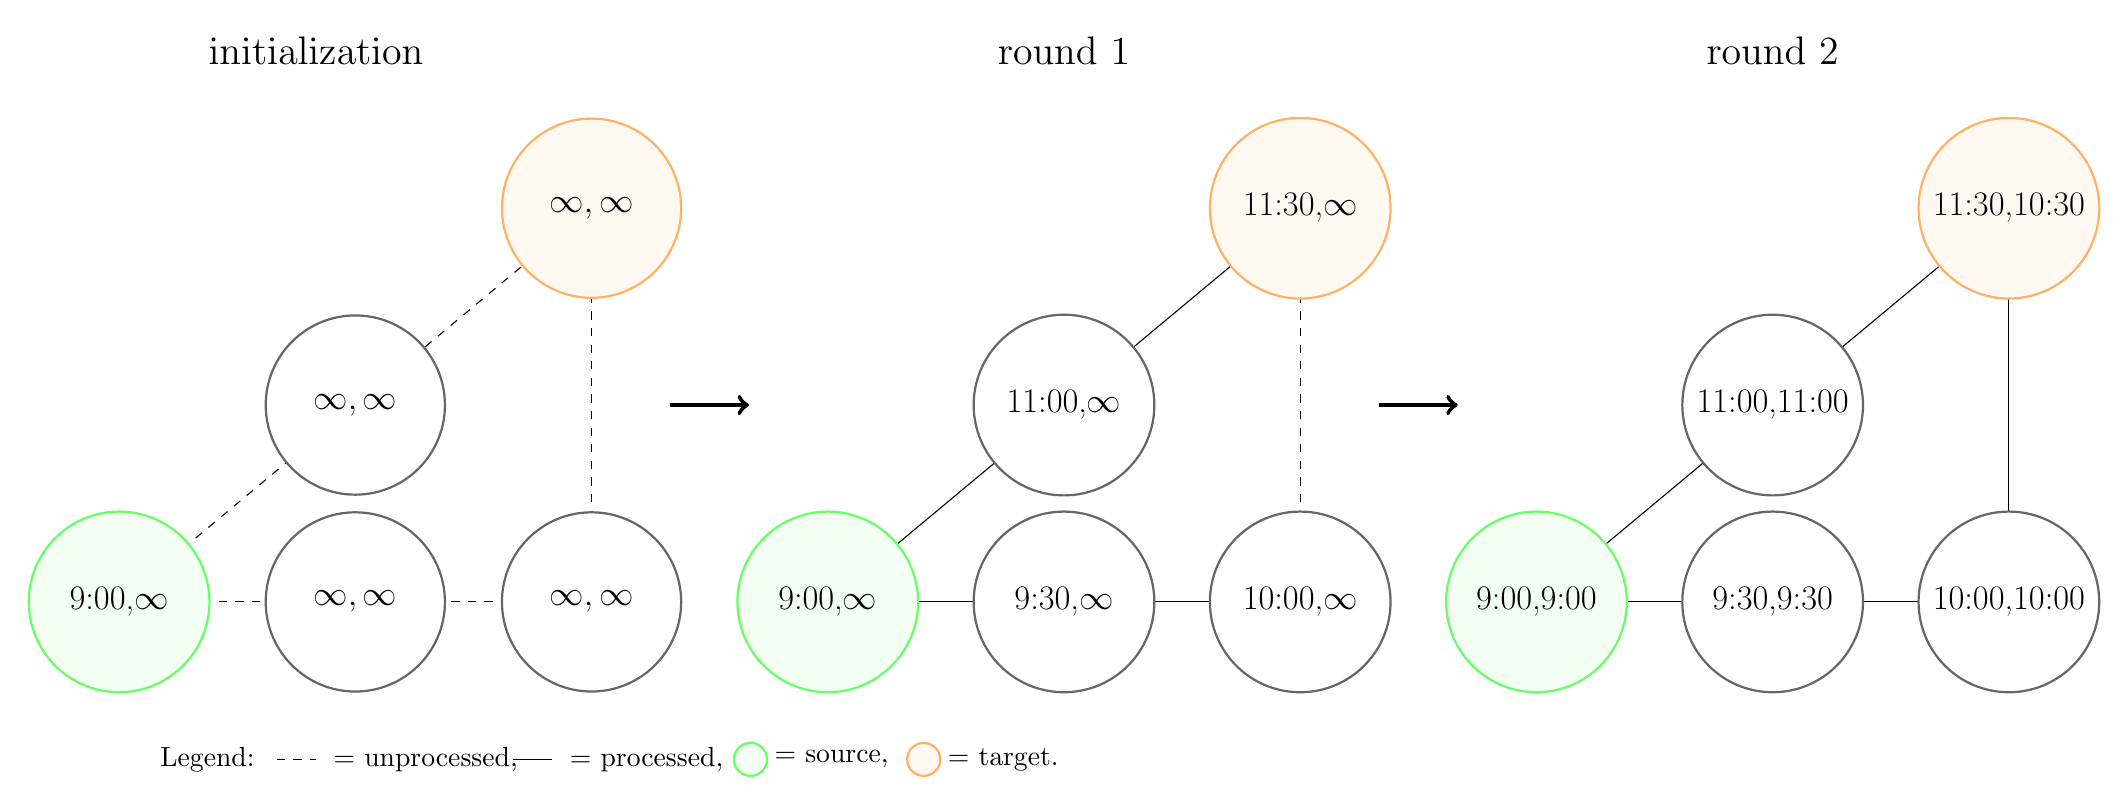
\begin{tikzpicture}[
roundnode/.style={circle, thick, minimum size=7mm, text width=3.5cm,align = center,scale=0.6,font=\huge},
green/.style={draw=green!60, fill=green!5},
orange/.style={draw=orange!60, fill=orange!5},
white/.style={draw=black!60, fill=white},
]
    \draw (0.4,-2) node[right=0] {Legend:};
    \draw [dashed](2,-2) -- (2.5,-2);
    \draw (2.6,-2) node[right=0] {= unprocessed,};
    \draw [](5,-2) -- (5.5,-2);
    \draw (5.6,-2) node[right=0] {= processed,};
    \draw (7.8,-2) node[roundnode,text width=0.4cm,green,right=0] {};
    \draw (8.2,-2) node[right=0] {= source,};
    \draw (10,-2) node[roundnode,text width=0.4cm,orange,right=0] {};
    \draw (10.4,-2) node[right=0] {= target.};
    
    \draw [dashed](0,0) -- (6,0);
    \draw [](9,0) -- (15,0);
    \draw [](18,0) -- (24,0);
    

    \draw [dashed](6,0) -- (6,5);
    \draw [dashed](15,0) -- (15,5);
    \draw [](24,0) -- (24,5);
    

    \draw [dashed](0,0) -- (6,5);
    \draw [](9,0) -- (15,5);
    \draw [](18,0) -- (24,5);
    
    \draw[->, ultra thick] (7,2.5) -- (8,2.5);
    \draw[->, ultra thick] (16,2.5) -- (17,2.5);
    
    \draw (0,0) node[roundnode,green] {9:00,$\infty$};
    \draw (3,0) node[roundnode,white] {$\infty,\infty$};
    \draw (6,0) node[roundnode,white] {$\infty,\infty$};
    \draw (3,2.5) node[roundnode,white] {$\infty,\infty$};
    \draw (6,5) node[roundnode,orange] {$\infty,\infty$};

    
    \draw (9,0) node[roundnode,green] {9:00,$\infty$};
    \draw (12,0) node[roundnode,white] {9:30,$\infty$};
    \draw (15,0) node[roundnode,white] {10:00,$\infty$};
    \draw (12,2.5) node[roundnode,white] {11:00,$\infty$};
    \draw (15,5) node[roundnode,orange] {11:30,$\infty$};

    
    \draw (18,0) node[roundnode,green] {9:00,9:00};
    \draw (21,0) node[roundnode,white] {9:30,9:30};
    \draw (24,0) node[roundnode,white] {10:00,10:00};
    \draw (21,2.5) node[roundnode,white] {11:00,11:00};
    \draw (24,5) node[roundnode,orange] {11:30,10:30};

    \draw (2.5,7) node[font=\Large] {initialization};
    \draw (12,7) node[font=\Large] {round 1};
    \draw (21,7) node[font=\Large] {round 2};
    \end{tikzpicture}
%
}%
    \caption{A small example using raptor, two rounds are show}
    \label{fig:raptor_example}
\end{figure}

\subsubsection{Hyper partitioning}
Hyper partitioning is a preprocessing-based acceleration technique for computing bi-criteria Pareto-optimal journeys in public transit networks, based on the well-known RAPTOR algorithm \cite{delling_round-based_2015}.
\subsubsection{Unrestricted footprints}
% TODO WIP
This work\cite{baum_ultra_2023} presents a new algorithm that uses trips (vehicles) and their transfers as its fundamental building blocks. Unlike existing algorithms, it does not assign labels to stops. Instead, trips are labelled with the stops at which they are boarded.
\subsection{After 2015}
The timeline in \autoref{fig:timeline} may you believe that no research was conducted on route planning algorithms. But this, of course, is not the case. However, most research focused on optimising existing algorithms like the scalable transfer patterns\cite{bast_scalable_2015} or ULTRA \cite{baum_ultra_2023}.

Others try to harvest the power of the Multicore CPU or the GPU. For example, the Earliest Arrival Time problem calculates the earliest arrival time starting from a source vertex and a departure time to all other reachable vertices in a temporal graph G. There also exists algorithms that use the multicore processors to get a reported 9.5 speedup over serial \glsxtrshort{csa} \cite{ni_parallel_2017}. Another paper proposes an algorithm/data structure for the GPU and reports speedups ranging from 2,29 to 59,09 over serial \glsxtrshort{csa} \cite{haryan_gpu_2020}.


\section{Data Models For public transport}\label{section:data_model_rel_work}

Since the ontologies for public transport are often based on existing data models and formats, it is interesting to have a small look at those data models.

A data model explicitly determines the structure of data. It is specified in a data modelling notation, which is often graphical.

\subsection{\glsfmtfull{gtfs}}
\glsxtrfull{gtfs} defines a common format for public transportation schedules and associated geographic information. “feeds” let public transit agencies publish their transit data. The developer can then write applications.

GTFS
“Downstream” 
+ widely used format for distributing timetables to third
  parties
- not all fare products and schemes are supported
- custom software needed for interpretation 
+ dataset available of NMBS

\subsubsection{\glsfmtshort{gtfs} feed}
A feed is a zip file containing CSV files but typically has the .txt extension. Some essential files include stops.txt, routes.txt, and trips.txt.

\subsection{Transmodel}
Transmodel is the European Standard “Public Transport Reference Data Model” by directive EN 12896.

Transmodel is the basis for defining exchange standards that enable the sharing and provision of accurate and interoperable public transport information across organisation- and system boundaries \cite{noauthor_transmodel_nodate}.

Transmodel provides matching definitions, structures, and semantics for PT data, not only for traditional modes but also for more modern modes like car-sharing or cycling. It also includes detailed information about stations and bus stops to ensure accessibility. In short, it has a comprehensive Conceptual Model covering multiple subdomains that support multi-modal, multi-operator transport systems.

All this is done with separation of concerns, meaning each part could be run independently but allow for their information to be combined. For example, physical stops (accessibility) and timetables. This is accomplished by using modern information architecture principles.

The standard also provides consistent terminology to avoid misunderstandings. Some of the important terms are:
\begin{itemize}
    \item \textbf{Scheduled stop points}: It is a place where passengers can board. The term does not care if it is a quay, bus stop, metro stop...
    \item \textbf{Physical stop place}: Is associated with a scheduled stop point.
    \item \textbf{Journey pattern}: It is a sequence of scheduled stop points as a pattern of working for a public transport vehicle. There is a separate journey pattern for each direction, but the same journey pattern may be used many times daily.
    \item \textbf{Vehicle journey or trip}: Unlike a journey pattern, a vehicle journey can only be used once a day since it is characterised by its departure time. It is the movement of a public transport vehicle from a start point to an endpoint of a journey pattern.
    \item \textbf{Service pattern}: A vehicle pattern that can carry passengers.
    \item \textbf{Dead run}: Opposite of service journey. A vehicle journey where passengers aren’t allowed to board. 
    \item \textbf{Block}: Describes the work for a vehicle on a day or part of a day. It typically starts and ends with a dead run. \autoref{fig:blocktransmodel} presents this concept visually.
    \item \textbf{Duty}: describes the work for a driver on a day. 
    \item \textbf{Day type}: Describes a logical type of day independent of any specific calendar date. 
\end{itemize}

The above concept has been simplified, and the Transmodel specification provides more in-depth definitions. These are accompanied by an entity-relationship model in \glsxtrfull{uml}.

\makeatletter
\begin{figure}[H]
\centering
\resizebox{.8\textwidth}{!}{%
    \begin{tikzpicture}[green/.style={draw=green!60, fill=green!5},
orange/.style={draw=orange!60, fill=orange!5},
white/.style={draw=black!60, fill=white},
roundnode/.style={circle, thick, minimum size=10mm,align = center,scale=0.6,font=\huge}
    ]
        
    % draw nodes
    \node[] (depot) at (-2,11) {Depot};
    \node[] (textiel) at (-2,8.5)  {Textiel-instituut};
    \node[] (Maaltebruggestraat) at (-2,6)  {Maaltebruggestraat};
    \node[] (Mariamiddelares) at (-2,3.5)  {Mariamiddelares};
    \node[] (expo) at (-2,1)  {Gent expo};
    \draw (depot) edge[opacity=0.1] (21,11);
    \draw (textiel) edge[opacity=0.1] (21,8.5);
    \draw (Maaltebruggestraat) edge[opacity=0.1] (21,6);
    \draw (Mariamiddelares) edge[opacity=0.1] (21,3.5);
    \draw (expo) edge[opacity=0.1] (21,1);
    %dead run 1
    \node[roundnode,white] (deadrun1) at (1,11) {};
    \node[roundnode,white] (deadrun2) at (2,8.5) {};
    \draw (deadrun1) edge[->] node[pos=0.5,right] {dead run} (deadrun2);

    % vehicle journey 1
    \node[roundnode,green] (vij1) at (3,8.5) {};
    \node[roundnode,green] (vij2) at (4,6) {};
    \node[roundnode,green] (vij3) at (5,3.5) {};
    \node[roundnode,green] (vij4) at (6,1) {};
    \draw (vij1) edge[->]  (vij2);
    \draw (vij2) edge[->] node[pos=0.5,right] {vehicle journey 1} (vij3);
    \draw (vij3) edge[->]  (vij4); 


    % vehicle journey 2
    \node[roundnode,orange] (vij21) at (10,8.5) {};
    \node[roundnode,orange] (vij22) at (9,6) {};
    \node[roundnode,orange] (vij23) at (8,3.5) {};
    \node[roundnode,orange] (vij24) at (7,1) {};
    \draw (vij21) edge[<-]  (vij22);
    \draw (vij22) edge[<-] node[pos=0.5,right] {vehicle journey 2} (vij23);
    \draw (vij23) edge[<-]  (vij24);


    % vehicle journey 3
    \node[roundnode,green] (vij31) at (11,8.5) {};
    \node[roundnode,green] (vij32) at (12,6) {};
    \node[roundnode,green] (vij33) at (13,3.5) {};
    \node[roundnode,green] (vij34) at (14,1) {};
    \draw (vij31) edge[->] (vij32);
    \draw (vij32) edge[->] node[pos=0.5,right] {vehicle journey 3} (vij33);
    \draw (vij33) edge[->] (vij34); 

    % vehicle journey 4
    \node[roundnode,orange] (vij41) at (18,8.5) {};
    \node[roundnode,orange] (vij42) at (17,6) {};
    \node[roundnode,orange] (vij43) at (16,3.5) {};
    \node[roundnode,orange] (vij44) at (15,1) {};
    \draw (vij41) edge[<-] (vij42);
    \draw (vij42) edge[<-] node[pos=0.5,right] {vehicle journey 4} (vij43);
    \draw (vij43) edge[<-] (vij44);

    %dead run 2
    \node[roundnode,white] (deadrun3) at (20,11) {};
    \node[roundnode,white] (deadrun4) at (19,8.5) {};
    \draw (deadrun3) edge[<-] node[pos=0.5,right] {dead run} (deadrun4);

    \draw (0,0) -- (0,12);
    \draw (0,0) edge[-{Latex[length=3mm,width=3mm]}] node[pos=0.5,below] {Time} (21,0);
    % Draw edges




    \end{tikzpicture}
    }
    \caption{This represents a block (defined above). It starts and ends with a dead run. It also uses two journey patterns (orange and green) and four service journeys.}
    \label{fig:blocktransmodel}
\end{figure}
\makeatother
\subsubsection{\glsfmtfull{ifopt}}
\glsxtrfull{ifopt} is a logical data model for the fixed objects relevant to public transport, particularly for stops and points of interest \cite{noauthor_ifopt_nodate}. It was also developed as a \glsxtrshort{cen} standard.

Transmodel v5.1 has been a fundamental input. IFOPT has been revised and incorporated into Transmodel v6 Part 2.
\subsubsection{Transmodel use in Belgium}
Transmodel is used by \glsxtrfull{stib} in the SPIDER STIB project. The new information system architecture is built upon the product MobilitX. MobilitX is a real-time, high-performance, reliable backbone dedicated to high-speed and massive transport information exchange \cite{noauthor_transmodel_nodate}.

Functionalities SPIDER STIB system implements the following parts of Transmodel \& \glsxtrshort{ifopt}:
\begin{itemize}
    \item Network topology
    \item Timetables
    \item Passenger Information
    \item Situation Management
    \item Accessibility
    \item Facility Management
\end{itemize}

\subsection{\glsfmtfull{netex}}
The NeTEx defines a standard for exchanging public transport passenger information data in XML format \cite{noauthor_downloads_nodate}.  

The standard is a subset of the \glsxtrfull{cen} conceptual model Transmodel and is divided into three parts. \begin{enumerate}
    \item Part one describes the fixed Network (stops, routes, lines, etc.).
    \item Part two is mainly focused on Timetables.
    \item Part three covers the fare exchange format.
\end{enumerate}

NeTEx deliverables comprise: \begin{enumerate}
    \item a CEN Specification document (in three parts)
    \item a data model in the standard UML modelling language
    \item an accompanying XML schema providing a formal electronic description that can be used by data processing software.
\end{enumerate}

Data in NeTEx format is encoded as XML documents that must conform precisely to the schema – standard XML validator tools can check conformance automatically. The schema can also be used to create bindings for different
programming languages, automating part of the implementation process for creating software that supports NeTEx
formats. 

A dataset of netex is available from the \glsxtrshort{nmbs} \cite{noauthor_use_nodate}. 

\subsubsection{Relation of \glsfmtshort{netex} with Transmodel}
As mentioned, \glsxtrshort{netex} is a subset of Transmodel, so it also covers a subset of the Transmodel functional domain:
\begin{itemize}
    \item The Network Topology
    \item Timing Information
    \item Vehicle Scheduling
    \item Fare Information
\end{itemize}
Transmodel itself has a much broader functional scope. In addition to \glsfmtshort{netex} it has Operations Monitoring and Control, Fare Management (sales, validation, control), Management Information
and Statistics, Driver Management, Driver Scheduling, Rostering, and Driving Personnel Disposition.
\subsubsection{Relation of \glsfmtshort{netex} with \glsfmtshort{gtfs}}

NeTEx is “upstream”, GTFS is “downstream”.

What is meant by downstream is that the primary focus \glsxtrshort{gtfs} was to exchange timetables to third parties. More specifically, it was developed to provide journey planning systems with data. 

NeTEx has a much broader scope. It is more upstream and intended for multi-sourced back-office use cases where data is generated, refined, and integrated.
\subsubsection{NETEX profiles}
Although NeTEx is a large standard, a NeTEx service needs only to implement the specific elements relevant to its business objectives \cite{noauthor_what_nodate}. 

Elements of the model that a service provider does not need can be ignored. If the service provider has a particular purpose, it will create a profile to identify the subset of elements that must be present. A machine-readable form of this profile may be made using the NeTEx TYPE OF FRAME element. This will still allow automatic validation.
\subsubsection{\glsfmtshort{netex} Belgium}
A \glsxtrshort{netex} profile for Belgium is called \glsxtrshort{netex}-Belgium. It describes how the terms should be used to describe the network topology and timetables of a public transport network. It is based on the \glsxtrfull{epip}. 

\section{Semantic Web and the role of Ontologies}\label{section:ontologies_rel_work}
\subsection{Semantic Web}
The semantic web can be seen as an extension of the current web and is a vision of Tim Berners-Lee, where web documents not only describe how to render data visually. The data is also annotated with terms to express how it should be interpreted. So, web documents also capture the meaning of the information.

The basis of the Semantic Web is linked data—structured data that is interlinked with other data. It builds upon existing protocols such as HTTP, RDF, and URIs.

There are four rules for linked data
\begin{enumerate}
    \item Use URIs as names for things

    \item Use HTTP URIs so that people can look up those names.

    \item When someone looks up a URI, provide useful information using the standards (RDF*, SPARQL)

    \item Include links to other URIs. so that they can discover more things.

\end{enumerate}

\subsubsection{Five star data}
Besides linked data, Sir Tim Berners-Lee also proposes a classification of data sources. It is a five-star deployment scheme for open data \cite{noauthor_5-star_nodate}.

\begin{enumerate}
    \item $\star$: Make your stuff available on the web (whatever format) under an open license
    \item $\star\star$ make it available as structured data (e.g., Excel instead of image scan of a table)
    \item $\star\star\star$ make it available in a non-proprietary open format (e.g., CSV instead of Excel)
    \item $\star\star\star\star$: use URIs to denote things so that people can point at your stuff
    \item $\star\star\star\star\star$:link your data to other data to provide context.
\end{enumerate}
\subsection{\glsfmtfull{rdf}}
\glsxtrfull{rdf} is an interchange data  model standardized by \glsfmtshort{w3c}. Originally meant for metadata, it has become a general method of exchanging graph data. An \glsfmtshort{rdf} dataset consists of default and named graphs. In turn, each graph consists of \glsfmtshort{rdf} triples. Each triple is made up of a subject, predicate and object. These are either a literal value, blank node or a named node represented by an \glsxtrfull{iri}.

\glsfmtshort{rdf} has multiple data serializations.
\begin{itemize}
    \item \textbf{Triple-base}: N-Triples, Turtle; N-Quads
    \item \textbf{JSON-based}: JSON-Ld
    \item \textbf{XML}: RDF/XML
\end{itemize}
There is also an embeddable variant for HTML called RDFa. 

\subsubsection{N-triples}
This serialisation only supports a default graph. A comment is made with a \#. \glsfmtshort{iri} is enclosed between < and >. literals are put between quotation marks. No prefixes are supported
\subsubsection{\glsfmtfull{turtle}}
This is a superset of N-Triples, which adds support for prefixes and contains a lot of syntactic sugar. 
\begin{itemize}

    \item \textbf{;} means reuse the subject.
    \item \textbf{,} means reuse the subject and predicate
    \item \textbf{@prefix name: <\glsfmtshort{iri}>} defines a new prefix. It has to be placed before any use.
    \item \textbf{\_:label} is a blank node label
    \item \textbf{[]} empty blank node, but properties can be defined by placing a predicate and object between the brackets.
    \item everything between \textbf{( )} is a list.
    
\end{itemize}
\begin{listing}[H]
    \inputminted[linenos,frame=single]{Turtle}{code/example_turtle.ttl}
    \caption{example of a turtle snippet describing a movie and a blank node representing a person who likes the movie.}
    \label{code: example:turtle}
\end{listing}
\subsubsection{\glsfmtfull{jsonld}}
\glsxtrfull{jsonld} is easy for both machines as developers since it is an interpretation on top of the \glsfmtshort{json} specification. The developer is unaware that it represents an \glsfmtshort{rdf} graph but still has a well-defined semantics. This is achieved by mapping each term to an \glsfmtshort{iri}. This mapping is provided by the term “@context” in the document itself. This context can be \glsfmtshort{iri}. 

The result of this mapping can be seen in \autoref{code: example:jsonmovie:expanded}, which is an expanded view of \autoref{code: example:jsonmovie}. Expansion is taking a JSON-LD document and applying a @context to expand all IRIs, types, and values so that the @context is no longer necessary. 

There is support for named graphs.
Terms are case-sensitive. 


\subsubsection{Keywords}
The most important keywords of \glsxtrshort{jsonld} are:
\begin{itemize}
    \item \textbf{@id}: Identifies resources with an \glsfmtshort{iri} or a blank node, a blank always starts with \textbf{\_:}.
    \item \textbf{@context}: To specify the context, 
    \item \textbf{@graph}: to express a named graph.
    \item \textbf{@language} String internalization, to specify the language for a particular string value.
\end{itemize}
The other keywords can be found at \url{https://www.w3.org/2018/jsonld-cg-reports/json-ld/#syntax-tokens-and-keywords}.

\begin{listing}[H]
    \inputminted[linenos,frame=single]{JSON-LD}{code/shema_movie_example_sita_raman.jsonld}
    \caption{This a small \glsfmtshort{jsonld} snippet that describes an schema.org/movie. This example can be parsed by the \glsxtrshort{json} playground \url{https://json-ld.org/playground/}}
    \label{code: example:jsonmovie}
\end{listing}

\begin{listing}[H]
    \inputminted[linenos,frame=single]{JSON-LD}{code/expanded_shema_movie.jsonld}
    \caption{This a small \glsfmtshort{jsonld} snippet that describes an schema.org/movie. After the process of expansion}
    \label{code: example:jsonmovie:expanded}
\end{listing}

\subsubsection{Advanced concepts}
\begin{itemize}
    \item \textbf{@vocab} keyword to use if all properties and types may come from the same vocabulary.
    \item \textbf{compact iri}: A compact IRI expresses an IRI using a prefix and suffix separated by a colon (:).
    \item \textbf{Embedding}: Embedding a node object as the property value of another node object.
\end{itemize}


\subsection{Ontologies}
The best definition of an ontology states: “An ontology is an explicit specification of a conceptualization” \cite{gruber_translation_1993}. Many ontologies exist, from basic to formal ontologies specified in highly expressive logic. In this thesis, we mainly use formal ontologies.

These ontologies play an essential role in the semantic web. 

A small study was conducted to find an ontology that best suited our needs. Many of the studied ontologies for transport are focused on specific use cases, for example, urban freight \cite{bouhana_ontology-based_2015}. They do not have a broad domain. 

\subsubsection{Ontologies of Wayfinding}
A Traveler’s Perspective \cite{timpf_ontologies_2002}, 2002
describes two ontologies of “wayfinding” with multiple transportation modes in an urban area based on two perspectives: the traveller and the public transportation system. A problem with the paper is that it only focuses on concepts and does not define any properties, relations or axioms. Also, it does not take in any hierarchy, as it is meant for urban areas only.

\subsubsection{An Ontology-based Public Transport Query System}

- server-side 

\subsubsection{A public transportation ontology to support user travel planning}
 A public transportation ontology to support user travel planning \cite{houda_public_2010} is a domain ontology with OWL 1.0 and was explicitly designed to support a planning tool on a country-wide scale. Validation was done by instantiating the ontology with actual instances examples of journeys. 


This is a relatively old ontology designed to be used with a user planning tool based on journey patterns. The ontology could support RAPTOR because it uses Journey patterns. Footpaths are supported in the form of infrastructure points.

Interestingly, they implemented a mobile application to plan tourist bus routes, but it relied on server-side queries. Other downsides are that there is no multi-modal support (only transport by bus) and no multi-operator support.

However, the ontology is not directly available; it is only provided as snippets in the paper. 
\subsubsection{Ontologies for transportation research: A survey  }
Using the study of transportation ontologies \cite{katsumi_ontologies_2018}, we only identify three ontologies that support journey patterns—two of which focus on city logistics and urban systems, which are different domains. The last ontology (Transportation ontology for content personalization) applies to PT, but the ontology is not directly available.

\subsubsection{Transmodel ontology}
This ontology is directly based on the concept of the Transmodel data model. An \glsxtrshort{cen} standard and European directives require every PT agent to be compatible with Transmodel, so an ontology aligned with Transmodel is interesting.

Further, the Transmodel ontology supports journey patterns. However, the ontology could be too broad, which leads to several potential problems. For example, it can make it hard to find relevant information, as the ontology may contain too many concepts and relationships that are not relevant. Furthermore, as the ontology may not be compatible with other ontologies used in those sources, integration from different sources can also be challenging.

\subsubsection{OSLO Mobility: Timetables and Planning}
The last ontology we looked at is the “OSLO Mobility - timetables and planning” \cite{noauthor_oslo_2023} ontology. The ontology is developed by \glsxtrfull{oslo}, a department of Data Flanders. It has been based on the EPIP profile. Since NETEX is based directly on the Transmodel ontology, the \glsxtrshort{oslo} mobility ontology is similar to the Transmodel ontology but is less broad than the Transmodel ontology.

The ontology describes the network topology and timetables of \glsfmtshort{pt} and is designed for Route planning, cartography, timetables and looking up lines/stops. This description is done in the form of lines. These lines can be grouped based on transport mode or be part of the network. These lines model a given Route with a direction and geometry by using points on the route. Another part describes the service that is offered on these points. A line follows a journey pattern; it explains all the points where the vehicle passes by but doesn’t necessarily stop. A service journey pattern describes service points where passengers can get off or on the vehicle. These points recalled planned stop points ( or in Dutch: GeplandeStoppunten). The description of a stopping point’s physical characteristics is linked. 

Timetables can be defined for these planned stop points. However, timetables can also be grouped by service journey.

A service journey’s day type can be defined because service journeys do not drive on each day of the week. 

\begin{listing}[H]
\inputminted[linenos,frame=single,breaklines]{jsonld}{code/oslo_example_line.jsonld}
\caption{A small example of \glsxtrshort{jsonld} snippet, a line is described which exists out of a route and is operated by an Operator. This is the actual correct snippet of our implementation and conforms to the \glsfmtshort{shacl}-file of \glsfmtshort{oslo}}
\label{code:
example:line}
\end{listing}


% TABLE
\begin{landscape}
\subsubsection{Overview}
% Please add the following required packages to your document preamble:
% \usepackage[table,xcdraw]{xcolor}
% Beamer presentation requires \usepackage{colortbl} instead of \usepackage[table,xcdraw]{xcolor}
\begin{table}[H]
\centering
\begin{tabular}{|l|l|l|l|l|l|l|}
\hline
\textbf{Ontology} &
  \textbf{\begin{tabular}[c]{@{}l@{}}Journey\\ patterns?\end{tabular}} &
  \textbf{\begin{tabular}[c]{@{}l@{}}Multi-\\ modal?\end{tabular}} &
  \textbf{\begin{tabular}[c]{@{}l@{}}Multi-\\ operator?\end{tabular}} &
  \textbf{\begin{tabular}[c]{@{}l@{}}Designed for use\\ with routeplanners\end{tabular}} &
  \textbf{\begin{tabular}[c]{@{}l@{}}directly available\\ for reuse?\end{tabular}} &
  \textbf{Citation} \\ \hline
\begin{tabular}[c]{@{}l@{}}Intoducing the public transport\\ domain to the web of data\end{tabular} &
  \cellcolor[HTML]{9AFF99}yes &
  \cellcolor[HTML]{9AFF99}yes &
  \cellcolor[HTML]{9AFF99}yes &
  \cellcolor[HTML]{9AFF99}yes &
  \cellcolor[HTML]{FD6864}no &
  \cite{benatallah_introducing_2014} \\ \hline
An Ontology-based public transport query system &
  \cellcolor[HTML]{FD6864}no &
  \cellcolor[HTML]{FD6864}no &
  \cellcolor[HTML]{9AFF99}yes &
  \cellcolor[HTML]{9AFF99}yes, query systems &
  \cellcolor[HTML]{FD6864}no &
  \cite{wang_ontology-based_2005} \\ \hline
iCity Ontology &
  \cellcolor[HTML]{9AFF99}yes &
  \cellcolor[HTML]{FD6864}no &
  \cellcolor[HTML]{FD6864}no &
  \cellcolor[HTML]{FD6864}no, urban systems &
  \cellcolor[HTML]{9AFF99}GitHub &
  \cite{noauthor_enterpriseintegrationlabicity_2023} \\ \hline
  
Genclon &
  \cellcolor[HTML]{9AFF99}yes &
  \cellcolor[HTML]{FD6864}no &
  \cellcolor[HTML]{FD6864}no &
  \cellcolor[HTML]{FD6864}no, city logistics &
  \cellcolor[HTML]{FD6864}no &
  \cite{anand_genclon_2012} \\ \hline
\begin{tabular}[c]{@{}l@{}}Transportation ontology\\ for content personalization\end{tabular} &
  \cellcolor[HTML]{9AFF99}yes &
  \cellcolor[HTML]{9AFF99}yes &
  \cellcolor[HTML]{9AFF99}yes &
  \cellcolor[HTML]{9AFF99}yes &
  \cellcolor[HTML]{FD6864}no &
  \cite{houda_public_2010} \\ \hline
linked-\glsxtrshort{gtfs} &
  \cellcolor[HTML]{9AFF99}yes &
  \cellcolor[HTML]{9AFF99}yes &
  \cellcolor[HTML]{9AFF99}yes &
  \cellcolor[HTML]{9AFF99}yes &
  \cellcolor[HTML]{9AFF99}yes &
  \cite{noauthor_opentransportlinked-gtfs_2023} \\ \hline
Transmodel ontology &
  \cellcolor[HTML]{9AFF99}yes &
  \cellcolor[HTML]{9AFF99}yes &
  \cellcolor[HTML]{9AFF99}yes &
  \cellcolor[HTML]{9AFF99}yes &
  \cellcolor[HTML]{9AFF99}GitHub &
  \cite{ruckhaus_applying_2023} \\ \hline
\begin{tabular}[c]{@{}l@{}}\glsxtrshort{oslo} Mobility:\\ Timetables and Planning\end{tabular} &
  \cellcolor[HTML]{9AFF99}yes &
  \cellcolor[HTML]{9AFF99}yes &
  \cellcolor[HTML]{9AFF99}yes &
  \cellcolor[HTML]{9AFF99}yes &
  \cellcolor[HTML]{9AFF99}yes &
  \cite{noauthor_oslo_2023} \\ \hline
\end{tabular}
\caption{An overview of the ontologies for }
\label{tab:my-table}
\end{table}
\end{landscape}


\subsection{\glsfmtfull{shacl}}
\glsxtrfull{shacl}\cite{noauthor_shapes_2017-1} is a language for describing and validating \glsxtrshort{rdf} graphs against a set of conditions. The conditions consist of shapes or shape graphs. \glsxtrshort{rdf} that are being validated are called data graphs. Since \glsxtrshort{shacl} can also be seen as a description of a correct Data graph, it can be used for code generation or user interface building.

The constraints described in the \glsxtrshort{shacl} example (\autoref{code:example:shacl})  for schema:movie are:
\begin{enumerate}
    \item Only one name per movie must be of type string.
    \item ContentRating and genre has to be of type xsd:string
    \item datePublished has to be of type schema:date
    \item No other properties can be defined, closed
\begin{listing}[H]
   \inputminted[linenos,frame=single]{turtle}{code/shacl_example.ttl}
    \caption{The \glsxtrshort{shacl} code can validate the \glsxtrshort{turtle} example given in \autoref{code:example:turtle}. An online tool to do this can be found at \url{https://shacl-playground.zazuko.com/}.}
    \label{code: example:shacl}
\end{listing}


    
\end{enumerate}

